\documentclass{standalone}
\usepackage{tikz}
\usetikzlibrary{patterns, positioning}

\begin{document}
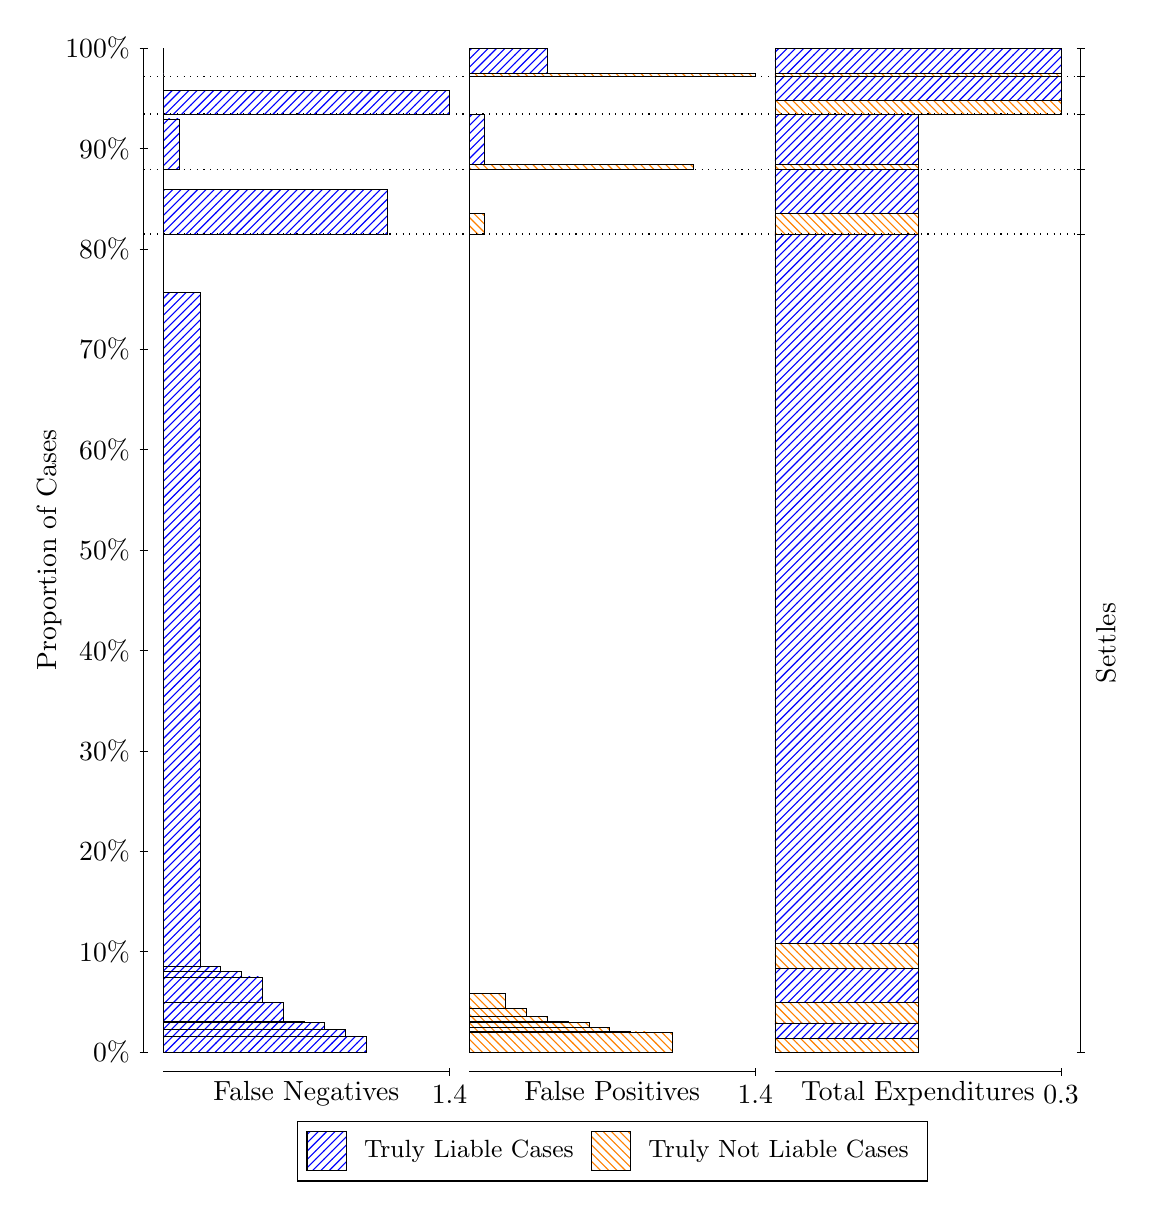
\begin{tikzpicture}
\draw[black, very thin] (1.5,1.75) -- (1.5,14.5);
\node[rotate=90, anchor=center] at (0.3, 8.125) {Proportion of Cases};
\draw[black, very thin] (1.45,1.75) -- (1.55,1.75);
\node[anchor=east] at (1.45, 1.75) {0\%};
\draw[black, very thin] (1.45,3.025) -- (1.55,3.025);
\node[anchor=east] at (1.45, 3.025) {10\%};
\draw[black, very thin] (1.45,4.3) -- (1.55,4.3);
\node[anchor=east] at (1.45, 4.3) {20\%};
\draw[black, very thin] (1.45,5.575) -- (1.55,5.575);
\node[anchor=east] at (1.45, 5.575) {30\%};
\draw[black, very thin] (1.45,6.85) -- (1.55,6.85);
\node[anchor=east] at (1.45, 6.85) {40\%};
\draw[black, very thin] (1.45,8.125) -- (1.55,8.125);
\node[anchor=east] at (1.45, 8.125) {50\%};
\draw[black, very thin] (1.45,9.4) -- (1.55,9.4);
\node[anchor=east] at (1.45, 9.4) {60\%};
\draw[black, very thin] (1.45,10.675) -- (1.55,10.675);
\node[anchor=east] at (1.45, 10.675) {70\%};
\draw[black, very thin] (1.45,11.95) -- (1.55,11.95);
\node[anchor=east] at (1.45, 11.95) {80\%};
\draw[black, very thin] (1.45,13.225) -- (1.55,13.225);
\node[anchor=east] at (1.45, 13.225) {90\%};
\draw[black, very thin] (1.45,14.5) -- (1.55,14.5);
\node[anchor=east] at (1.45, 14.5) {100\%};

\draw[black, very thin] (13.4,1.75) -- (13.4,14.5);
\draw[black, very thin] (13.35,1.75) -- (13.45,1.75);
\node[anchor=west] at (13.35, 1.75) {};
\draw[black, very thin] (13.35,12.138) -- (13.45,12.138);
\node[anchor=west] at (13.35, 12.138) {};
\draw[black, very thin] (13.35,12.961) -- (13.45,12.961);
\node[anchor=west] at (13.35, 12.961) {};
\draw[black, very thin] (13.35,13.662) -- (13.45,13.662);
\node[anchor=west] at (13.35, 13.662) {};
\draw[black, very thin] (13.35,14.141) -- (13.45,14.141);
\node[anchor=west] at (13.35, 14.141) {};
\draw[black, very thin] (13.35,14.5) -- (13.45,14.5);
\node[anchor=west] at (13.35, 14.5) {};

\draw[black, very thin, pattern color=blue, pattern=north east lines] (1.75,1.75) rectangle (4.3264,1.9434);
\draw[black, very thin, pattern color=blue, pattern=north east lines] (1.75,1.9434) rectangle (4.0621,2.0377);
\draw[black, very thin, pattern color=blue, pattern=north east lines] (1.75,2.0377) rectangle (3.7979,2.1243);
\draw[black, very thin, pattern color=blue, pattern=north east lines] (1.75,2.1243) rectangle (3.5336,2.137);
\draw[black, very thin, pattern color=blue, pattern=north east lines] (1.75,2.137) rectangle (3.2694,2.3828);
\draw[black, very thin, pattern color=blue, pattern=north east lines] (1.75,2.3828) rectangle (3.0052,2.7034);
\draw[black, very thin, pattern color=blue, pattern=north east lines] (1.75,2.7034) rectangle (2.7409,2.771);
\draw[black, very thin, pattern color=blue, pattern=north east lines] (1.75,2.771) rectangle (2.4767,2.8376);
\draw[black, very thin, pattern color=blue, pattern=north east lines] (1.75,2.8376) rectangle (2.2124,11.393);
\draw[black, very thin, pattern color=orange, pattern=north west lines] (1.75,11.393) rectangle (1.75,12.138);
\draw[black, very thin, pattern color=blue, pattern=north east lines] (1.75,12.138) rectangle (4.5906,12.701);
\draw[black, very thin, pattern color=orange, pattern=north west lines] (1.75,12.701) rectangle (1.75,12.961);
\draw[black, very thin, pattern color=blue, pattern=north east lines] (1.75,12.961) rectangle (1.9482,13.6);
\draw[black, very thin, pattern color=orange, pattern=north west lines] (1.75,13.6) rectangle (1.75,13.662);
\draw[black, very thin, pattern color=blue, pattern=north east lines] (1.75,13.662) rectangle (5.3833,13.966);
\draw[black, very thin, pattern color=orange, pattern=north west lines] (1.75,13.966) rectangle (1.75,14.141);
\draw[black, very thin, pattern color=orange, pattern=north west lines] (1.75,14.141) rectangle (1.75,14.174);
\draw[black, very thin, pattern color=blue, pattern=north east lines] (1.75,14.174) rectangle (1.75,14.5);
\draw[black, very thin, pattern color=orange, pattern=north west lines] (5.6333,1.75) rectangle (8.2097,1.9973);
\draw[black, very thin, pattern color=orange, pattern=north west lines] (5.6333,1.9973) rectangle (7.9455,2.0053);
\draw[black, very thin, pattern color=orange, pattern=north west lines] (5.6333,2.0053) rectangle (7.6812,2.0138);
\draw[black, very thin, pattern color=orange, pattern=north west lines] (5.6333,2.0138) rectangle (7.417,2.0632);
\draw[black, very thin, pattern color=orange, pattern=north west lines] (5.6333,2.0632) rectangle (7.1527,2.1271);
\draw[black, very thin, pattern color=orange, pattern=north west lines] (5.6333,2.1271) rectangle (6.8885,2.1306);
\draw[black, very thin, pattern color=orange, pattern=north west lines] (5.6333,2.1306) rectangle (6.8885,2.1358);
\draw[black, very thin, pattern color=orange, pattern=north west lines] (5.6333,2.1358) rectangle (6.6242,2.206);
\draw[black, very thin, pattern color=orange, pattern=north west lines] (5.6333,2.206) rectangle (6.36,2.303);
\draw[black, very thin, pattern color=orange, pattern=north west lines] (5.6333,2.303) rectangle (6.0958,2.4954);
\draw[black, very thin, pattern color=blue, pattern=north east lines] (5.6333,2.4954) rectangle (5.6333,12.138);
\draw[black, very thin, pattern color=orange, pattern=north west lines] (5.6333,12.138) rectangle (5.8315,12.398);
\draw[black, very thin, pattern color=blue, pattern=north east lines] (5.6333,12.398) rectangle (5.6333,12.961);
\draw[black, very thin, pattern color=orange, pattern=north west lines] (5.6333,12.961) rectangle (8.4739,13.023);
\draw[black, very thin, pattern color=blue, pattern=north east lines] (5.6333,13.023) rectangle (5.8315,13.662);
\draw[black, very thin, pattern color=orange, pattern=north west lines] (5.6333,13.662) rectangle (5.6333,13.837);
\draw[black, very thin, pattern color=blue, pattern=north east lines] (5.6333,13.837) rectangle (5.6333,14.141);
\draw[black, very thin, pattern color=orange, pattern=north west lines] (5.6333,14.141) rectangle (9.2667,14.174);
\draw[black, very thin, pattern color=blue, pattern=north east lines] (5.6333,14.174) rectangle (6.6242,14.5);
\draw[black, very thin, pattern color=orange, pattern=north west lines] (9.5167,1.75) rectangle (11.333,1.9259);
\draw[black, very thin, pattern color=blue, pattern=north east lines] (9.5167,1.9259) rectangle (11.333,2.1195);
\draw[black, very thin, pattern color=orange, pattern=north west lines] (9.5167,2.1195) rectangle (11.333,2.3758);
\draw[black, very thin, pattern color=blue, pattern=north east lines] (9.5167,2.3758) rectangle (11.333,2.815);
\draw[black, very thin, pattern color=orange, pattern=north west lines] (9.5167,2.815) rectangle (11.333,3.1282);
\draw[black, very thin, pattern color=blue, pattern=north east lines] (9.5167,3.1282) rectangle (11.333,12.138);
\draw[black, very thin, pattern color=orange, pattern=north west lines] (9.5167,12.138) rectangle (11.333,12.398);
\draw[black, very thin, pattern color=blue, pattern=north east lines] (9.5167,12.398) rectangle (11.333,12.961);
\draw[black, very thin, pattern color=orange, pattern=north west lines] (9.5167,12.961) rectangle (11.333,13.023);
\draw[black, very thin, pattern color=blue, pattern=north east lines] (9.5167,13.023) rectangle (11.333,13.662);
\draw[black, very thin, pattern color=orange, pattern=north west lines] (9.5167,13.662) rectangle (13.15,13.837);
\draw[black, very thin, pattern color=blue, pattern=north east lines] (9.5167,13.837) rectangle (13.15,14.141);
\draw[black, very thin, pattern color=orange, pattern=north west lines] (9.5167,14.141) rectangle (13.15,14.174);
\draw[black, very thin, pattern color=blue, pattern=north east lines] (9.5167,14.174) rectangle (13.15,14.5);
\draw[black, dotted] (1.5,12.138) -- (13.4,12.138);
\draw[black, dotted] (1.5,12.961) -- (13.4,12.961);
\draw[black, dotted] (1.5,13.662) -- (13.4,13.662);
\draw[black, dotted] (1.5,14.141) -- (13.4,14.141);
\draw[black, very thin] (1.75,1.5) -- (5.3833,1.5);
\node[anchor=north] at (3.5667, 1.5) {False Negatives};
\draw[black, very thin] (5.3833,1.45) -- (5.3833,1.55);
\node[anchor=north] at (5.3833, 1.45) {1.4};

\draw[black, very thin] (5.6333,1.5) -- (9.2667,1.5);
\node[anchor=north] at (7.45, 1.5) {False Positives};
\draw[black, very thin] (9.2667,1.45) -- (9.2667,1.55);
\node[anchor=north] at (9.2667, 1.45) {1.4};

\draw[black, very thin] (9.5167,1.5) -- (13.15,1.5);
\node[anchor=north] at (11.333, 1.5) {Total Expenditures};
\draw[black, very thin] (13.15,1.45) -- (13.15,1.55);
\node[anchor=north] at (13.15, 1.45) {0.3};

\node[black, centered, rotate=90] at (13.72, 6.9442) {Settles};





\draw (7.449999999999999,1.5) node[draw=none] (baseCoordinate) {};
\begin{scope}[align=center]
        \matrix[scale=0.5, draw=black, below=0.5cm of baseCoordinate, nodes={draw}, column sep=0.1cm]{
            \node[rectangle, draw, minimum width=0.5cm, minimum height=0.5cm, pattern=north east lines, pattern color=blue] {}; &
            \node[draw=none, font=\small] (B) {Truly Liable Cases}; &
            \node[rectangle, draw, minimum width=0.5cm, minimum height=0.5cm, pattern=north west lines, pattern color=orange] {}; &
            \node[draw=none, font=\small] (B) {Truly Not Liable Cases}; \\
            };
\end{scope}

\end{tikzpicture}
\end{document}